The NINJA-1 project was a huge success in bringing the numerical
relativity and gravitational-wave astronomy communities together.  The
project also resulted in several intriguing qualitative results.
However, it only began the process of testing detection and parameter
estimation pipelines against realistic signals.  The follow-up
project, NINJA-2, is ongoing as of the time of writing.  NINJA-2 aims
to remove some of the shortcomings of NINJA-1 and allow quantitative
studies of the behaviors of pipelines in varying regions of signal
parameter space.  Specifically, NINJA-2 addresses issues with both the
waveform submissions and the noise used to construct the data sets.

\section{Hybrid pN/NR waveforms}

NINJA-1 had an open policy towards waveforms submission in order to
encourage wide participation.  This meant there were no requirements
on either waveform quality or length.  The lack of quality
requirements can be seen in some of the waveforms in
figure~\ref{fig:NR-Reh22} .  There may also be less visible
implications, as there was no requirement to perform the kind of
convergence testing reported in
section~\cite{sec:PNNRHybridWaveform}, although such validation is
typically done by numerical relativistists.  The loose requirements
limited the conclusions that could be drawn, for example it makes it
difficult to say whether an injection was missed due to the parameters
of the signal or an unintended feature of the waveform.

The lack of length requirement limited the available mass range to $M
< 36 \msun$ for reasons that can be seen in
figure~\ref{fig:StildesAndInitialPSD}.   Had the waveform in that plot
not had a post-Newtonian component, the NR component to the right of
the triangles would have had to be placed below 40 Hz in order to
prevent turning on in-band.  This mass range limited the tests that
could be done, for example it entirely excludes the standard CBC
low-mass pipeline.

To address these issues NINJA-2 specifies the following minimal
requirements~\cite{ninja2-wiki}.  The raw numerical simulation should
include at least five orbits of usable data before merger (i.e., not
counting bursts of junk radiation or other significant noise).  Given
the computation cost of extending the NR waveforms, we instead require
stitching to a post-Newtonian inspiral approximant, which should be
performed at a GW frequency of $M\omega ≤ 0.075$, where $M\omega$ is
the frequency of the $(l = 2, m = \pm 2)$ harmonic. The full waveform
should be long enough to be entirely within the sensitivity bands of
LIGO and Virgo down to $10 \msun$ with a lower cutoff frequency of 10
Hz, which corresponds to a starting GW frequency of $M\omega = 0.003$.
The numerical-waveform (before any hybridization) amplitude should be
accurate to within 5\%, and the phase (as a function of GW frequency)
should have an accumulated uncertainty over the entire inspiral,
merger and ringdown, of no more than 0.5 radian. The PN approximants
used for hybridization should ideally use the highest PN orders
available, both in phase and amplitude.  

These minimal accuracy requirements are motivated by the results of
the Samurai project~\cite{Hannam:2009hh}, and studies performed in
preparation for the NR-AR collaboration project~\cite{ninja-wiki}.
The question of how many NR cycles are needed in order to produce a
robust waveform is an area of current research. \Note{cite Ilana}.

The NINJA-2 project encourages although does not require the addition
of higher-order modes.  We chose to restrict attention to non-spinning
waveforms and waveforms with spins aligned or anti-aligned with the
orbital angular momentum.  There are sufficient open questions
regarding these restricted cases to make this analysis interesting,
without adding the additional complications on both the NR and data
analysis sides associated with precession. 

A total of 60 waveforms from 8 groups were contributed, these are
summarized in tables ~\ref{tab:ninja2_bam}, \ref{tab:ninja2_fau},
\ref{tab:ninja2_gatech}, \ref{tab:ninja2_lean},
\ref{tab:ninja2_llama}, \ref{tab:ninja2_rit}, \ref{tab:ninja2_spec},
\ref{tab:ninja2_uiuc} and a map of the parameter values is shown in
figure~\ref{f:ninja2_param_map}.

\begin{table}
\begin{center}
\begin{tabular}{|l|r|r|r|l|c|}
\hline
Run & $q$ & Spin1${}_z$ & Spin2${}_z$ & pN Approx. & Refs \\
\hline
BAM\_D10spp85\_80.T4.hyb.n2 & 1 & 0.85 & 0.85 & TaylorT4 & \cite{Hannam:2007wf,Brugmann:2008zz} \\
BAM\_D10spp85\_80.T1.hyb.n2 & 1 & 0.85 & 0.85 & TaylorT1 & \cite{Hannam:2007wf,Brugmann:2008zz} \\
BAM\_D125smm50Nep\_80.T1.hyb.n2 & 1 & -0.50 & -0.50 & TaylorT1 & \cite{Hannam:2007wf,Brugmann:2008zz} \\
BAM\_D125smm50Nep\_80.T4.hyb.n2 & 1 & -0.50 & -0.50 & TaylorT4 & \cite{Hannam:2007wf,Brugmann:2008zz} \\
BAM\_D13smm75Nep\_96.T4.hyb.n2 & 1 & -0.75 & -0.75 & TaylorT4 & \cite{Hannam:2007wf,Brugmann:2008zz} \\
BAM\_D13smm75Nep\_96.T1.hyb.n2 & 1 & -0.75 & -0.75 & TaylorT1 & \cite{Hannam:2007wf,Brugmann:2008zz} \\
BAM\_D13smm85Nep\_88.T4.hyb.n2 & 1 & -0.85 & -0.85 & TaylorT4 & \cite{Hannam:2007wf,Brugmann:2008zz} \\
BAM\_D13smm85Nep\_88.T1.hyb.n2 & 1 & -0.85 & -0.85 & TaylorT1 & \cite{Hannam:2007wf,Brugmann:2008zz} \\
BAM\_D11spp50\_96.T4.hyb.n2 & 1 & 0.50 & 0.50 & TaylorT4 & \cite{Hannam:2007wf,Brugmann:2008zz} \\
BAM\_D11spp50\_96.T1.hyb.n2 & 1 & 0.50 & 0.50 & TaylorT1 & \cite{Hannam:2007wf,Brugmann:2008zz} \\
BAM\_D10spp75\_80.T1.hyb.n2 & 1 & 0.75 & 0.75 & TaylorT1 & \cite{Hannam:2007wf,Brugmann:2008zz} \\
BAM\_D10spp75\_80.T4.hyb.n2 & 1 & 0.75 & 0.75 & TaylorT4 & \cite{Hannam:2007wf,Brugmann:2008zz} \\
BAM\_D12smm25Nep\_80.T4.hyb.n2 & 1 & -0.25 & -0.25 & TaylorT4 & \cite{Hannam:2007wf,Brugmann:2008zz} \\
BAM\_D12smm25Nep\_80.T1.hyb.n2 & 1 & -0.25 & -0.25 & TaylorT1 & \cite{Hannam:2007wf,Brugmann:2008zz} \\
BAM\_EP\_um4\_D10-n96.T4.hyb.n2 & 4 & 0.00 & 0.00 & TaylorT4 & \cite{Hannam:2007wf,Brugmann:2008zz} \\
BAM\_EP\_um4\_D10-n96.T1.hyb.n2 & 4 & 0.00 & 0.00 & TaylorT1 & \cite{Hannam:2007wf,Brugmann:2008zz} \\
BAM\_um3\_88.T4.hyb.n2 & 3 & 0.00 & 0.00 & TaylorT4 & \cite{Hannam:2007wf,Brugmann:2008zz} \\
BAM\_um3\_88.T1.hyb.n2 & 3 & 0.00 & 0.00 & TaylorT1 & \cite{Hannam:2007wf,Brugmann:2008zz} \\
BAM\_um2\_88.T1.hyb.n2 & 2 & 0.00 & 0.00 & TaylorT1 & \cite{Hannam:2007wf,Brugmann:2008zz} \\
BAM\_um2\_88.T4.hyb.n2 & 2 & 0.00 & 0.00 & TaylorT4 & \cite{Hannam:2007wf,Brugmann:2008zz} \\
BAM\_R6\_PN\_80.T1.hyb.n2 & 1 & 0.00 & 0.00 & TaylorT1 & \cite{Hannam:2007wf,Brugmann:2008zz} \\
BAM\_R6\_PN\_80.T4.hyb.n2 & 1 & 0.00 & 0.00 & TaylorT4 & \cite{Hannam:2007wf,Brugmann:2008zz} \\
BAM\_D12spp25\_96.T4.hyb.n2 & 1 & 0.25 & 0.25 & TaylorT4 & \cite{Hannam:2007wf,Brugmann:2008zz} \\
BAM\_D12spp25\_96.T1.hyb.n2 & 1 & 0.25 & 0.25 & TaylorT1 & \cite{Hannam:2007wf,Brugmann:2008zz} \\
BAM\_q2a0a025\_T\_96\_344.T1.hyb.n2.bbh & 2 & 0.25 & 0.00 & {} & \cite{,Brugmann:2008zz} \\
BAM\_q2a0a025\_T\_96\_344.T4.hyb.n2.bbh & 2 & 0.25 & 0.00 & {} & \cite{,Brugmann:2008zz} \\
\hline
\end{tabular}
\end{center}
\caption[BAM submissions to NINJA-2]{
\label{tab:ninja2_bam}
BAM submissions to NINJA-2}
\end{table}

\begin{table}
\begin{center}
\begin{tabular}{|l|r|r|r|l|c|}
\hline
Run & $q$ & Spin1${}_z$ & Spin2${}_z$ & pN Approx. & Refs \\
\hline
BAM\_hybrid\_om0.025etmq3S0.4- & 3 & 0.40 & 0.60 & TaylorT4 & \cite{none,???} \\
0\_0\_S0.6\_0\_0\_72 &  &  &  &  &  \\
\hline
\end{tabular}
\end{center}
\caption[FAU submissions to NINJA-2]{
\label{tab:ninja2_fau}
FAU submissions to NINJA-2}
\end{table}

\begin{table}
\begin{center}
\begin{tabular}{|l|r|r|r|l|c|}
\hline
Run & $q$ & Spin1${}_z$ & Spin2${}_z$ & pN Approx. & Refs \\
\hline
MayaKranc\_D12\_a0.00\_m129\_nj & 1 & 0.00 & 0.00 & TaylorT4 & \cite{,} \\
MayaKranc\_D10\_a0.90\_m129\_nj & 1 & 0.90 & 0.90 & TaylorT4 & \cite{,} \\
MayaKranc\_D10\_a0.20\_m77\_nj & 1 & 0.20 & 0.20 & TaylorT4 & \cite{,} \\
MayaKranc\_D10\_a0.60\_m77\_nj & 1 & 0.60 & 0.60 & TaylorT4 & \cite{,} \\
MayaKranc\_D12\_a0.60\_m103\_nj & 1 & 0.60 & 0.60 & TaylorT4 & \cite{,} \\
MayaKranc\_Sp02py0935th90\_gr & 1 & 0.80 & 0.00 & TaylorT4 & \cite{,} \\
MayaKranc\_D12\_a0.80\_m103\_nj & 1 & 0.80 & 0.80 & TaylorT4 & \cite{,} \\
MayaKranc\_D12\_a0.00\_q2\_m90\_nj & 2 & 0.00 & 0.00 & TaylorT4 & \cite{,} \\
MayaKranc\_D11\_a0.20\_q2\_m90\_nj & 2 & 0.02 & 0.09 & TaylorT4 & \cite{,} \\
MayaKranc\_D10\_a0.40\_m90\_nj & 1 & 0.40 & 0.40 & TaylorT4 & \cite{,} \\
MayaKranc\_D10\_a0.80\_m90\_nj & 1 & 0.80 & 0.80 & TaylorT4 & \cite{,} \\
MayaKranc\_D12\_a0.40\_m103\_nj & 1 & 0.40 & 0.40 & TaylorT4 & \cite{,} \\
MayaKranc\_D12\_a0.20\_m103\_nj & 1 & 0.20 & 0.20 & TaylorT4 & \cite{,} \\
\hline
\end{tabular}
\end{center}
\caption[GATech submissions to NINJA-2]{
\label{tab:ninja2_gatech}
GATech submissions to NINJA-2}
\end{table}

\begin{table}
\begin{center}
\begin{tabular}{|l|r|r|r|l|c|}
\hline
Run & $q$ & Spin1${}_z$ & Spin2${}_z$ & pN Approx. & Refs \\
\hline
dq4 & 4 & 0.00 & 0.00 & TaylorT1 & \cite{,Sperhake:2006cy} \\
\hline
\end{tabular}
\end{center}
\caption[LEAN submissions to NINJA-2]{
\label{tab:ninja2_lean}
LEAN submissions to NINJA-2}
\end{table}

\begin{table}
\begin{center}
\begin{tabular}{|l|r|r|r|l|c|}
\hline
Run & $q$ & Spin1${}_z$ & Spin2${}_z$ & pN Approx. & Refs \\
\hline
Llama\_d550-h64-Hybrid & 1 & 0.00 & 0.00 & 3.5pNTaylorF2 & \cite{Reisswig:2009rx,Reisswig:2009rx} \\
Llama\_d4d4-q1--D10-h64-r250.T4.hybrid & 1 & -0.40 & -0.40 & TaylorT4 & \cite{Pollney:2010hs,Pollney:2009yz,} \\
Llama\_d4d4-q1--D10-h64-r250.T1.hybrid & 1 & -0.40 & -0.40 & TaylorT1 & \cite{Pollney:2010hs,Pollney:2009yz,} \\
Llama\_u4u4-q1--D8-h64-r250.T1.hybrid & 1 & 0.40 & 0.40 & TaylorT1 & \cite{Pollney:2010hs,Pollney:2009yz,} \\
Llama\_u4u4-q1--D8-h64-r250.T4.hybrid & 1 & 0.40 & 0.40 & TaylorT4 & \cite{Pollney:2010hs,Pollney:2009yz,} \\
Llama\_d5q2-h016-Hybrid & 2 & 0.00 & 0.00 & 3.5pNTaylorF2 & \cite{,Reisswig:2009rx} \\
Llama\_u2u2-q1--D8-h64-r250.T1.hybrid & 1 & 0.20 & 0.20 & TaylorT1 & \cite{Pollney:2010hs,Pollney:2009yz,} \\
Llama\_u2u2-q1--D8-h64-r250.T4.hybrid & 1 & 0.20 & 0.20 & TaylorT4 & \cite{Pollney:2010hs,Pollney:2009yz,} \\
Llama\_d2d2-q1--D10-h64-r250.T1.hybrid & 1 & -0.20 & -0.20 & TaylorT1 & \cite{Pollney:2010hs,Pollney:2009yz,} \\
Llama\_d2d2-q1--D10-h64-r250.T4.hybrid & 1 & -0.20 & -0.20 & TaylorT4 & \cite{Pollney:2010hs,Pollney:2009yz,} \\
\hline
\end{tabular}
\end{center}
\caption[Llama submissions to NINJA-2]{
\label{tab:ninja2_llama}
Llama submissions to NINJA-2}
\end{table}

\begin{table}
\begin{center}
\begin{tabular}{|l|r|r|r|l|c|}
\hline
Run & $q$ & Spin1${}_z$ & Spin2${}_z$ & pN Approx. & Refs \\
\hline
LazEV\_D8.4\_10to1\_nj\_hybrid & 10 & 0.00 & 0.00 & TaylorT4 & \cite{Campanelli:2005dd} \\
\hline
\end{tabular}
\end{center}
\caption[RIT submissions to NINJA-2]{
\label{tab:ninja2_rit}
RIT submissions to NINJA-2}
\end{table}

\begin{table}
\begin{center}
\begin{tabular}{|l|r|r|r|l|c|}
\hline
Run & $q$ & Spin1${}_z$ & Spin2${}_z$ & pN Approx. & Refs \\
\hline
SpEC\_q6s0 & 6 & 0.00 & 0.00 & TaylorT1 & \cite{SpECWebsite} \\
SpEC\_q4s0 & 4 & 0.00 & 0.00 & TaylorT2 & \cite{SpECWebsite} \\
SpEC\_EqualMassAntiAlignedSpins & 1 & -0.44 & -0.44 & NA & \cite{chu-2009,SpECWebsite} \\
SpEC\_q1s-0.95 & 1 & -0.95 & -0.95 & TaylorT1 & \cite{SpECWebsite} \\
SpEC\_q2s0 & 2 & 0.00 & 0.00 & TaylorT2 & \cite{SpECWebsite} \\
SpEC\_EqualMassAlignedSpins & 1 & 0.44 & 0.44 & NA & \cite{chu-2009,SpECWebsite} \\
SpEC\_q3s0 & 3 & 0.00 & 0.00 & TaylorT2 & \cite{SpECWebsite} \\
SpEC\_EqualMassNonspinning & 1 & 0.00 & 0.00 & TaylorT4 & \cite{Scheel:2008rj,SpECWebsite} \\
\hline
\end{tabular}
\end{center}
\caption[SpEC submissions to NINJA-2]{
\label{tab:ninja2_spec}
SpEC submissions to NINJA-2}
\end{table}

\begin{table}
\begin{center}
\begin{tabular}{|l|r|r|r|l|c|}
\hline
Run & $q$ & Spin1${}_z$ & Spin2${}_z$ & pN Approx. & Refs \\
\hline
UIUC\_spin\_-0.25\_om0.0528\_22-HYBRID & 1 & -0.25 & -0.25 & NA & \cite{none} \\
UIUC\_spin\_0.85\_om0.0536\_22-HYBRID & 1 & 0.85 & 0.85 & NA & \cite{none} \\
\hline
\end{tabular}
\end{center}
\caption[UIUC submissions to NINJA-2]{
\label{tab:ninja2_uiuc}
UIUC submissions to NINJA-2}
\end{table}


\begin{figure}
  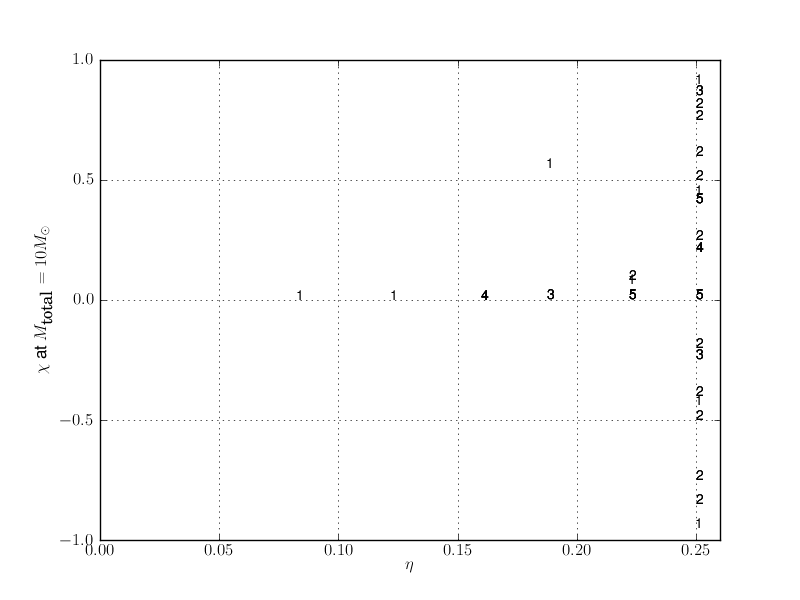
\includegraphics[width=\linewidth]{figures/ninja2/ninja2_cat.png}
  \caption[Parameters of the NINJA-2 submissions]{
  \label{f:ninja2_param_map}
Parameters of the NINJA-2 hybrid waveform submissions showing the
symmetric mass ratio $\eta=m_1 m_2 /(m_1+m_2)^2$ and dimensionless
spin parameter $\chi=(S_1/m_1 + S_2/m_2)/(m_1+m_2)$ after scaling the
waveforms to a total mass of 10 $\msun$.  The numbers indicate how
many distinct waveforms with the specified parameters were submitted.}
\end{figure}%

\subsection{Verifying the hybrid waveforms}

Each NR group verified that their waveforms met the minimum NINJA-2
requirements before submission.  Once submitted, a series of checks
were performed in order to validate the waveforms against each other.

In the first stage the post-Newtonian expressions and codes were
compared against each other and the literature.  This required several
iterations, but resulted in a set of codes in various languages that
produce waveforms that all agree in both phase and amplitude. 

In the second stage the complete hybrid waveforms were examined.
We first plotted the last 40 cycles of each waveform -- enough to
include the full NR portion, the hybridization region, and some of the
pN portion -- and looked for any anomalies such as those present in
some of the NINJA-1 waveforms in figure~\ref{fig:NR-Reh22}.  A few such
features were indeed visible, spotting them in this way allowed them
to be corrected.  One example is shown in figure (\Note{show the dq4
waveform before and after, note this was due to a problem integrating
psi4, and discuss this stage a little in the NR section of chapter
3}).

The amplitude of the Fourier transform of the complete waveforms were
also plotted.  This analysis also revealed unphysical features, 
primarily due to hybridization.  An example is shown in
figure~\ref{f:ninja2_freq_hybrids}, which shows a visible ``kink'' in
the waveform at the hybridization frequency, which vanishes after the
waveform was reconstructed.

\begin{figure}
  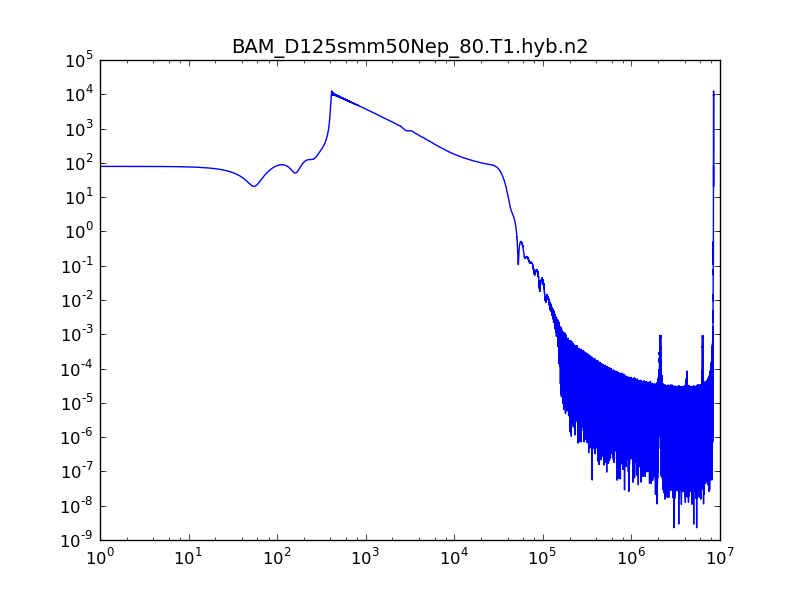
\includegraphics[width=0.5\linewidth]{figures/ninja2/bam_d125smm50nep_80_t1_hyb_n2_amp.png}
  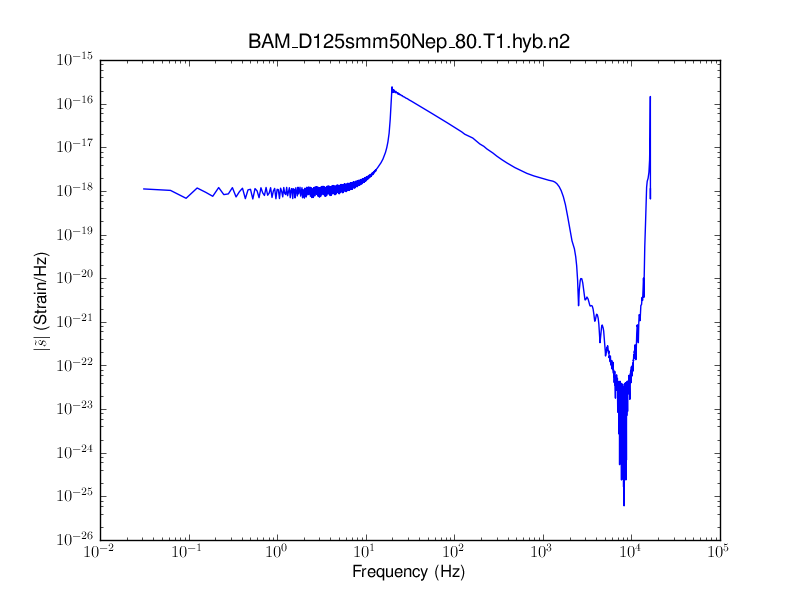
\includegraphics[width=0.5\linewidth]{figures/ninja2/bam_d125smm50nep_80_t1_hyb_n2_amp_v2.png}
  \caption[Frequency-domain hybrid NINJA-2 waveforms]{
  \label{f:ninja2_freq_hybrids}
Fourier amplitude of the (2,2) mode of a sample NINJA-2 hybrid
waveform from the BAM/AEI group.  The waveform has been scaled to 10
$\msun$ and placed 1 Mpc from the detector to give it physical units.
\Note{I need to dig up the old version of the waveform and remake it
with the new code} The waveform on the left is the version
initially submitted, note there is a visible ``kink'' in the waveform
at the hybridization frequency.  The waveform on the right has been
re-hybridized and there is no longer a visible kink.  This feature did
not show up in the time domain view of the waveform.}
\end{figure}%

Finally, the waveforms were compared against each other using standard
data-analysis techniques, in particular the overlap defined in
section~\ref{sec:search_matchfilter}. \Note{Should I include the
definition here (and in other chapters that use it) to remind the
reader, and refer back to this section for more details?}.

\begin{figure}
  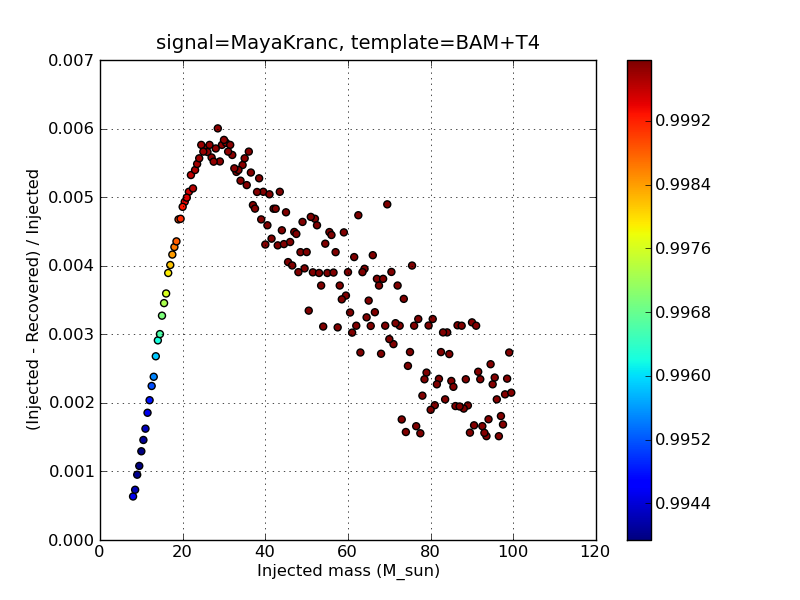
\includegraphics[width=0.5\linewidth]{figures/ninja2/maya_bamt4_max_over_m}
  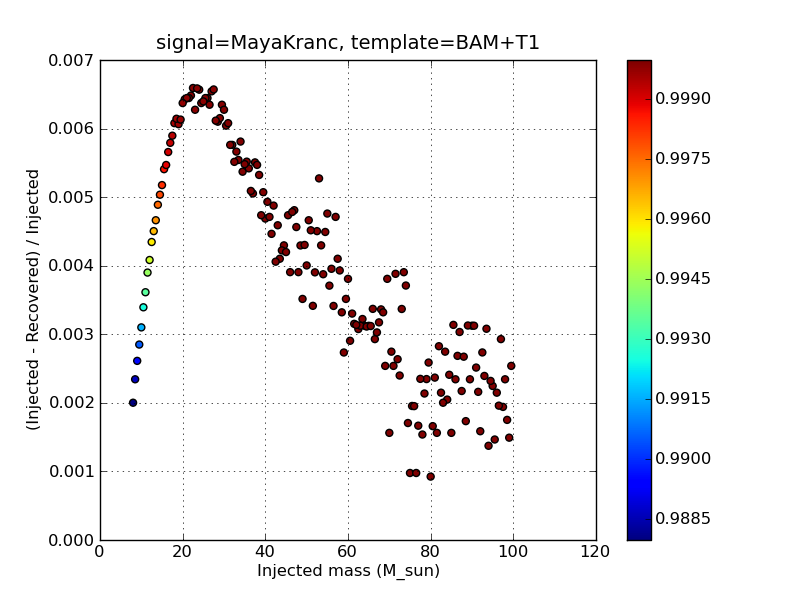
\includegraphics[width=0.5\linewidth]{figures/ninja2/maya_bamt1_max_over_m}
  \caption[Overlaps between NINJA-2 submissions maximized over mass]{
  \label{f:ninja2_max_over_mass_bam}
Overlaps between the equal-mass, non-spinning MayaKranc waveform taken
as the signal, and the equal-mass, non-spinning BAM waveform
hybridized with TaylorT4 (left) and TaylorT1 (right) taken as
templates.  Maximization is done over mass, as well as time and phase.
Note the lower overall overlaps and mass bias at the low-mass end,
where the two pN waveforms dominate the overlap.}
\end{figure}%


\section{Construction of the NINJA-2 data set}

\begin{figure}
  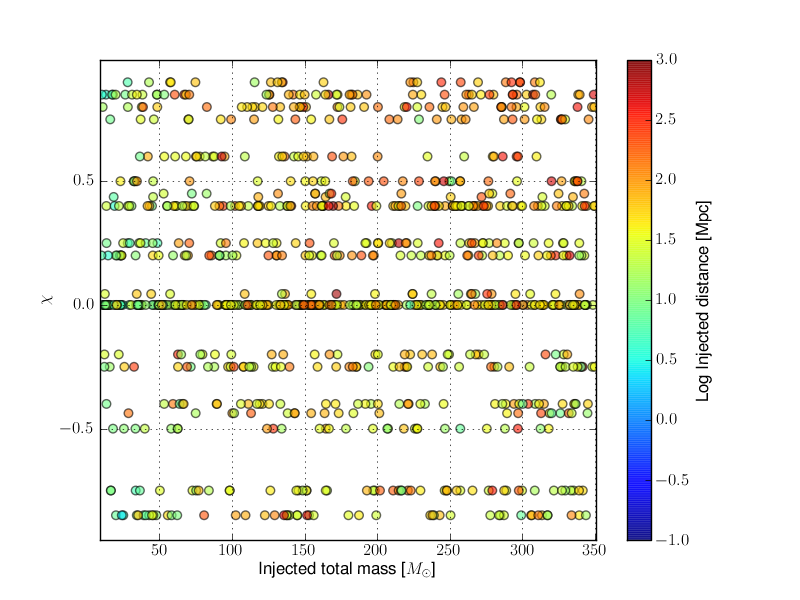
\includegraphics[width=\linewidth]{figures/ninja2/ninja2_dataset.png}
  \caption[Parameters of the NINJA-2 two-month data set]{
  \label{f:ninja2_dataset}
Distribution of mass, spin and distance parameters in the two-month,
Gaussian-noise data set.
}
\end{figure}%



% TODO:
% make tables of submissions
% plot of paramater space in eta, chi scaled to 10 M
% plot of injection set (use chi instead of sum of magnitudes)
% text
% results
% explain move to 16384 (plot showing aliasing)

